

\tikzset{every picture/.style={line width=0.75pt}} %set default line width to 0.75pt        

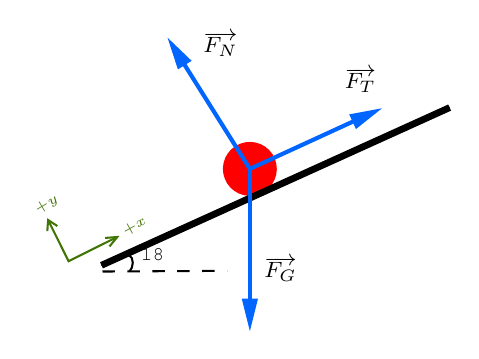
\begin{tikzpicture}[x=0.75pt,y=0.75pt,yscale=-1,xscale=1]
	%uncomment if require: \path (0,300); %set diagram left start at 0, and has height of 300

	%Shape: Ellipse [id:dp1428949648769431] 
	\draw  [color={rgb, 255:red, 255; green, 0; blue, 0 }  ,draw opacity=1 ][fill={rgb, 255:red, 254; green, 0; blue, 0 }  ,fill opacity=1 ] (149.04,183.11) .. controls (147.8,176.33) and (152.3,169.83) .. (159.09,168.59) .. controls (165.87,167.35) and (172.38,171.85) .. (173.61,178.64) .. controls (174.85,185.42) and (170.35,191.93) .. (163.56,193.16) .. controls (156.78,194.4) and (150.28,189.9) .. (149.04,183.11) -- cycle ;
	%Shape: Rectangle [id:dp48287918810377195] 
	\draw   (89.84,226.09) -- (256.64,150.53) -- (256.96,151.22) -- (90.15,226.78) -- cycle ;
	%Shape: Rectangle [id:dp005233673921997584] 
	\draw   (90.15,226.78) -- (256.96,151.22) -- (257.27,151.91) -- (90.46,227.47) -- cycle ;
	%Shape: Rectangle [id:dp9526931686132831] 
	\draw   (90.46,227.47) -- (257.27,151.91) -- (257.58,152.6) -- (90.77,228.16) -- cycle ;

	%Straight Lines [id:da8350690671631047] 
	\draw [color={rgb, 255:red, 1; green, 101; blue, 255 }  ,draw opacity=1 ][line width=1.5]    (161.33,180.88) -- (161.33,255.01) ;
	\draw [shift={(161.33,259.01)}, rotate = 270] [fill={rgb, 255:red, 1; green, 101; blue, 255 }  ,fill opacity=1 ][line width=0.08]  [draw opacity=0] (15.6,-3.9) -- (0,0) -- (15.6,3.9) -- cycle    ;
	%Straight Lines [id:da1062981577052522] 
	\draw [color={rgb, 255:red, 1; green, 101; blue, 255 }  ,draw opacity=1 ][line width=1.5]    (161.33,180.88) -- (123.79,121.05) ;
	\draw [shift={(121.67,117.67)}, rotate = 57.89] [fill={rgb, 255:red, 1; green, 101; blue, 255 }  ,fill opacity=1 ][line width=0.08]  [draw opacity=0] (15.6,-3.9) -- (0,0) -- (15.6,3.9) -- cycle    ;
	%Straight Lines [id:da21972886949175963] 
	\draw [color={rgb, 255:red, 1; green, 101; blue, 255 }  ,draw opacity=1 ][line width=1.5]    (161.33,180.88) -- (221.36,153.33) ;
	\draw [shift={(225,151.67)}, rotate = 155.36] [fill={rgb, 255:red, 1; green, 101; blue, 255 }  ,fill opacity=1 ][line width=0.08]  [draw opacity=0] (15.6,-3.9) -- (0,0) -- (15.6,3.9) -- cycle    ;
	%Shape: Right Angle [id:dp7929492774408056] 
	\draw  [color={rgb, 255:red, 65; green, 117; blue, 5 }  ,draw opacity=1 ][line width=0.75]  (97.31,213.73) -- (73.99,225.35) -- (64.15,205.57) ;
	\draw  [color={rgb, 255:red, 65; green, 117; blue, 5 }  ,draw opacity=1 ] (63.75,210.84) -- (64.11,205.52) -- (68.6,208.42) ;
	\draw  [color={rgb, 255:red, 65; green, 117; blue, 5 }  ,draw opacity=1 ] (91.56,214.16) -- (97.45,213.7) -- (93.7,218.23) ;

	%Curve Lines [id:da5437896212575373] 
	\draw    (103,222.33) .. controls (105.67,223.67) and (105.33,228.33) .. (103.33,230.33) ;
	%Straight Lines [id:da9621621519167294] 
	\draw  [dash pattern={on 4.5pt off 4.5pt}]  (90.33,230.33) -- (150.33,230) ;

	% Text Node
	\draw (166.85,221.91) node [anchor=north west][inner sep=0.75pt]  [font=\footnotesize] [align=left] {$\displaystyle \overrightarrow{F_{G}}$};
	% Text Node
	\draw (205.56,130.62) node [anchor=north west][inner sep=0.75pt]  [font=\footnotesize] [align=left] {$\displaystyle \overrightarrow{F_{T}}$};
	% Text Node
	\draw (137.43,113.35) node [anchor=north west][inner sep=0.75pt]  [font=\footnotesize,color={rgb, 255:red, 0; green, 0; blue, 0 }  ,opacity=1 ] [align=left] {$\displaystyle \overrightarrow{F_{N}}$};
	% Text Node
	\draw (107.33,218) node [anchor=north west][inner sep=0.75pt]  [font=\scriptsize] [align=left] {{\fontfamily{pcr}\selectfont 18}$\displaystyle \degree $};
	% Text Node
	\draw (97.11,208.66) node [anchor=north west][inner sep=0.75pt]  [font=\tiny,color={rgb, 255:red, 65; green, 117; blue, 5 }  ,opacity=1 ,rotate=-331] [align=left] {$\displaystyle +x$};
	% Text Node
	\draw (54.78,198.23) node [anchor=north west][inner sep=0.75pt]  [font=\tiny,color={rgb, 255:red, 65; green, 117; blue, 5 }  ,opacity=1 ,rotate=-329.58] [align=left] {$\displaystyle +y$};


\end{tikzpicture}